\documentclass[twocolumn, a4paper]{article}
\usepackage{graphicx}
\usepackage{float}

%opening
\title{COMP 5411 Programming Assignment 1 Report }
\author{Mu Cong DING}

\begin{document}

\maketitle

\begin{abstract}
This is the report for the programming assignment 1 of COMP 5411 by Mu Cong DING.
\end{abstract}

\section{Laplacian Smoothing on Bunny}
\begin{figure}[H]
	\centering
	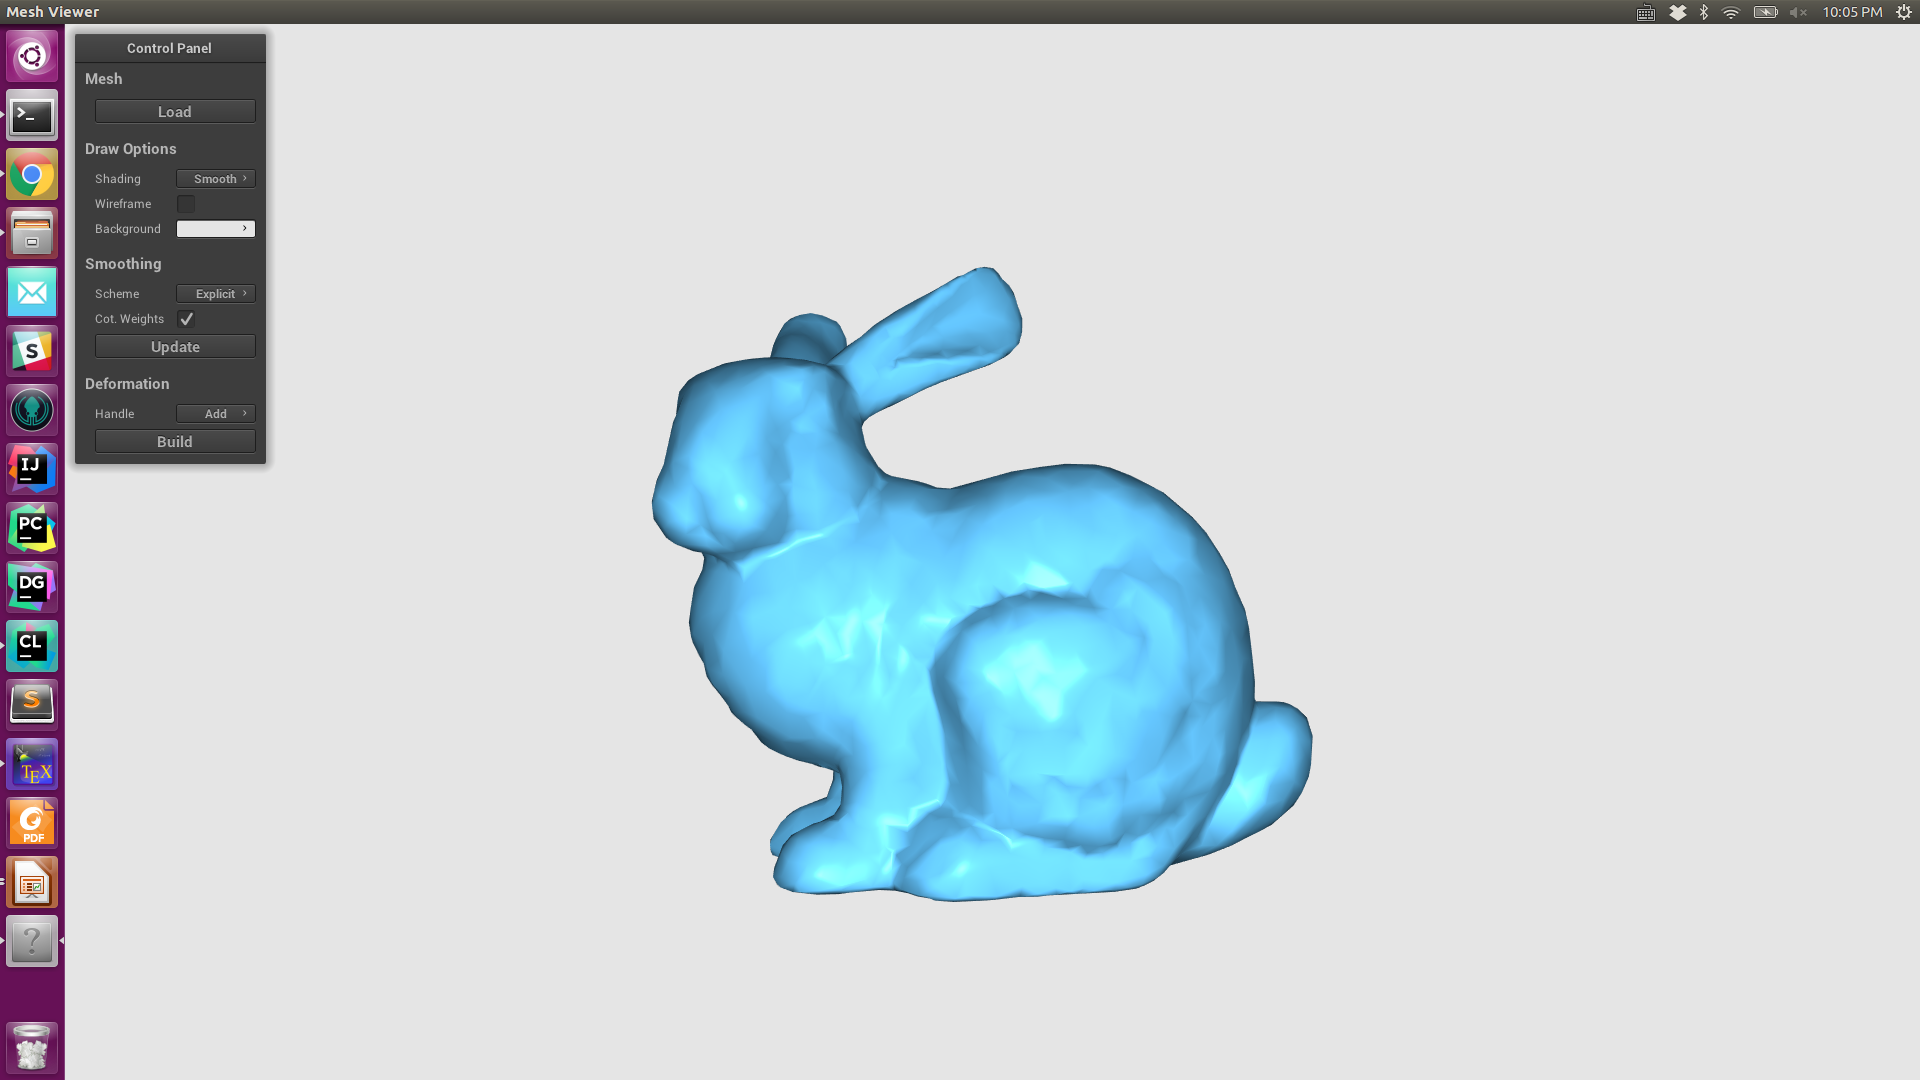
\includegraphics[width=1.0\linewidth]{bunny.png}
	\caption{original bunny}
\end{figure}
\begin{figure}[H]
	\centering
	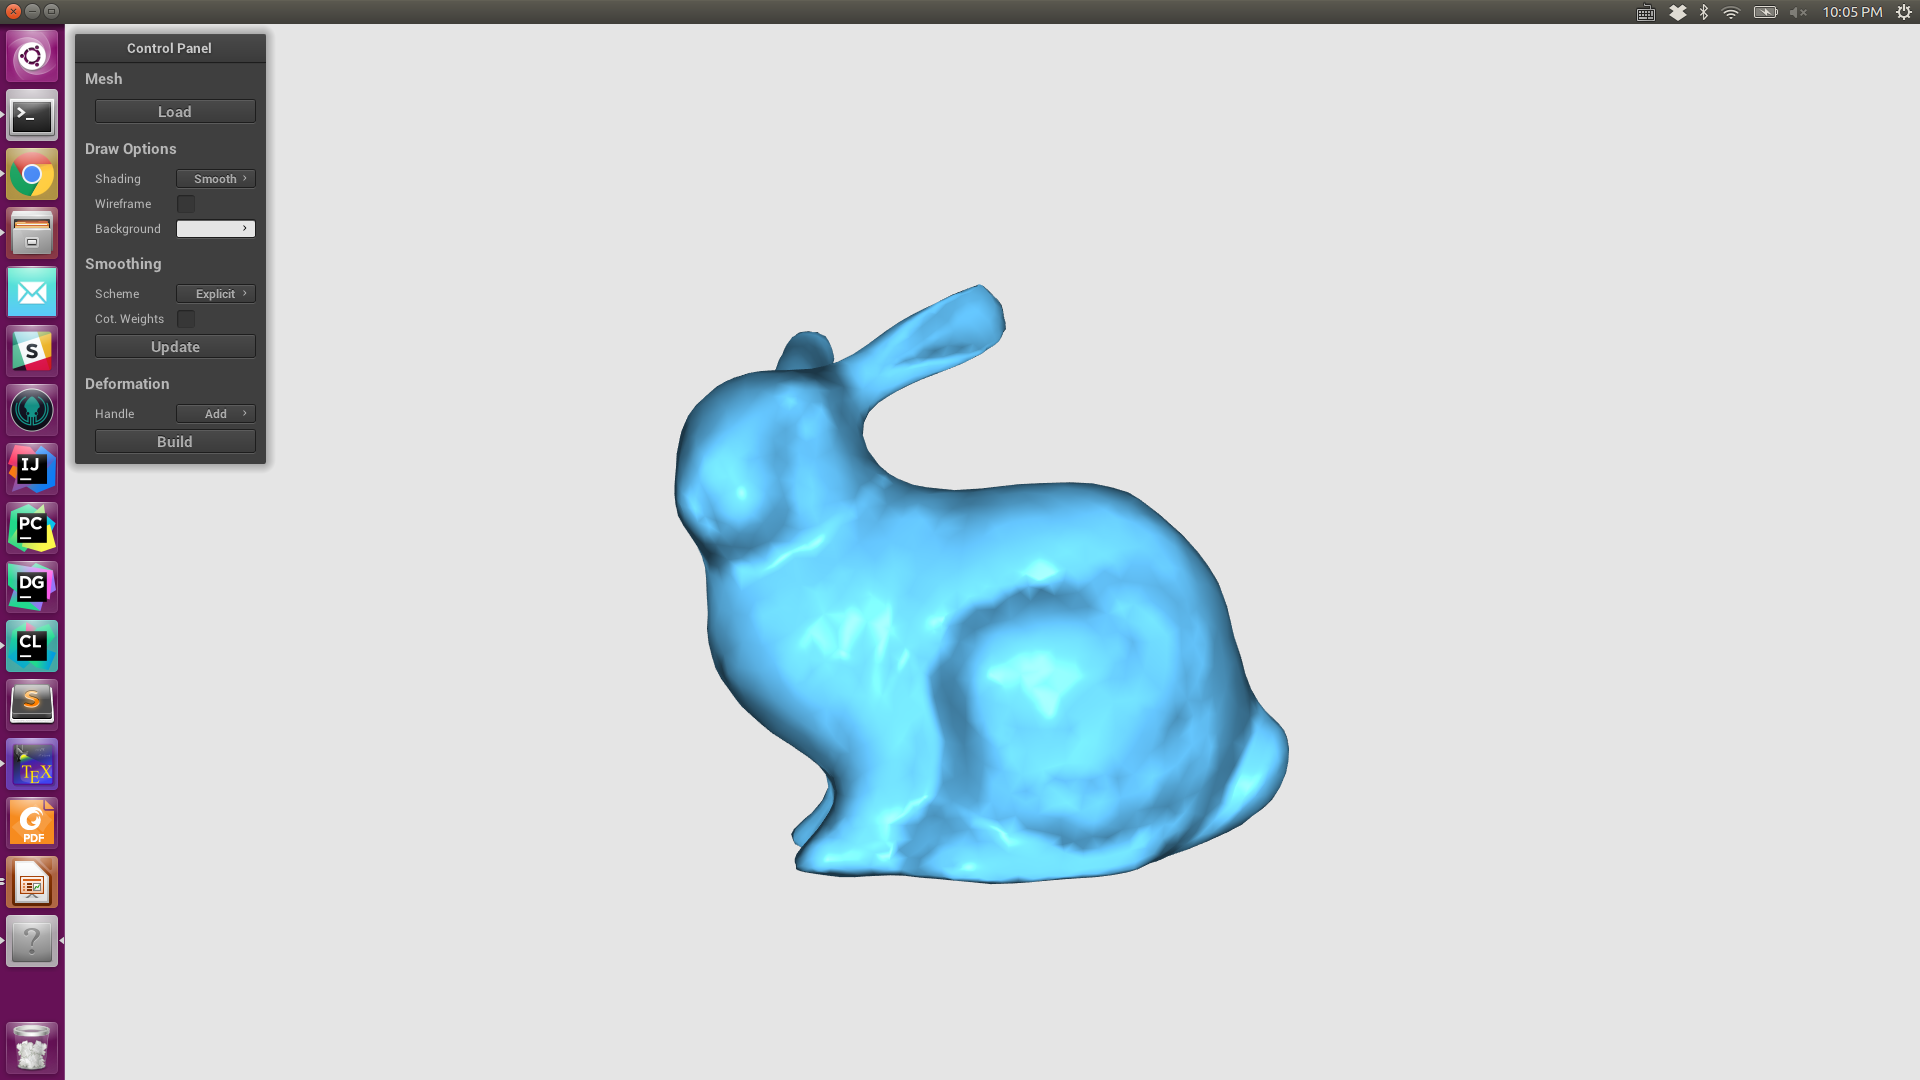
\includegraphics[width=1.0\linewidth]{bunny_en_15.png}
	\caption{bunny after explicit unweighted laplacian smoothing 15 times with $\lambda=0.5$.}
\end{figure}
\begin{figure}[H]
	\centering
	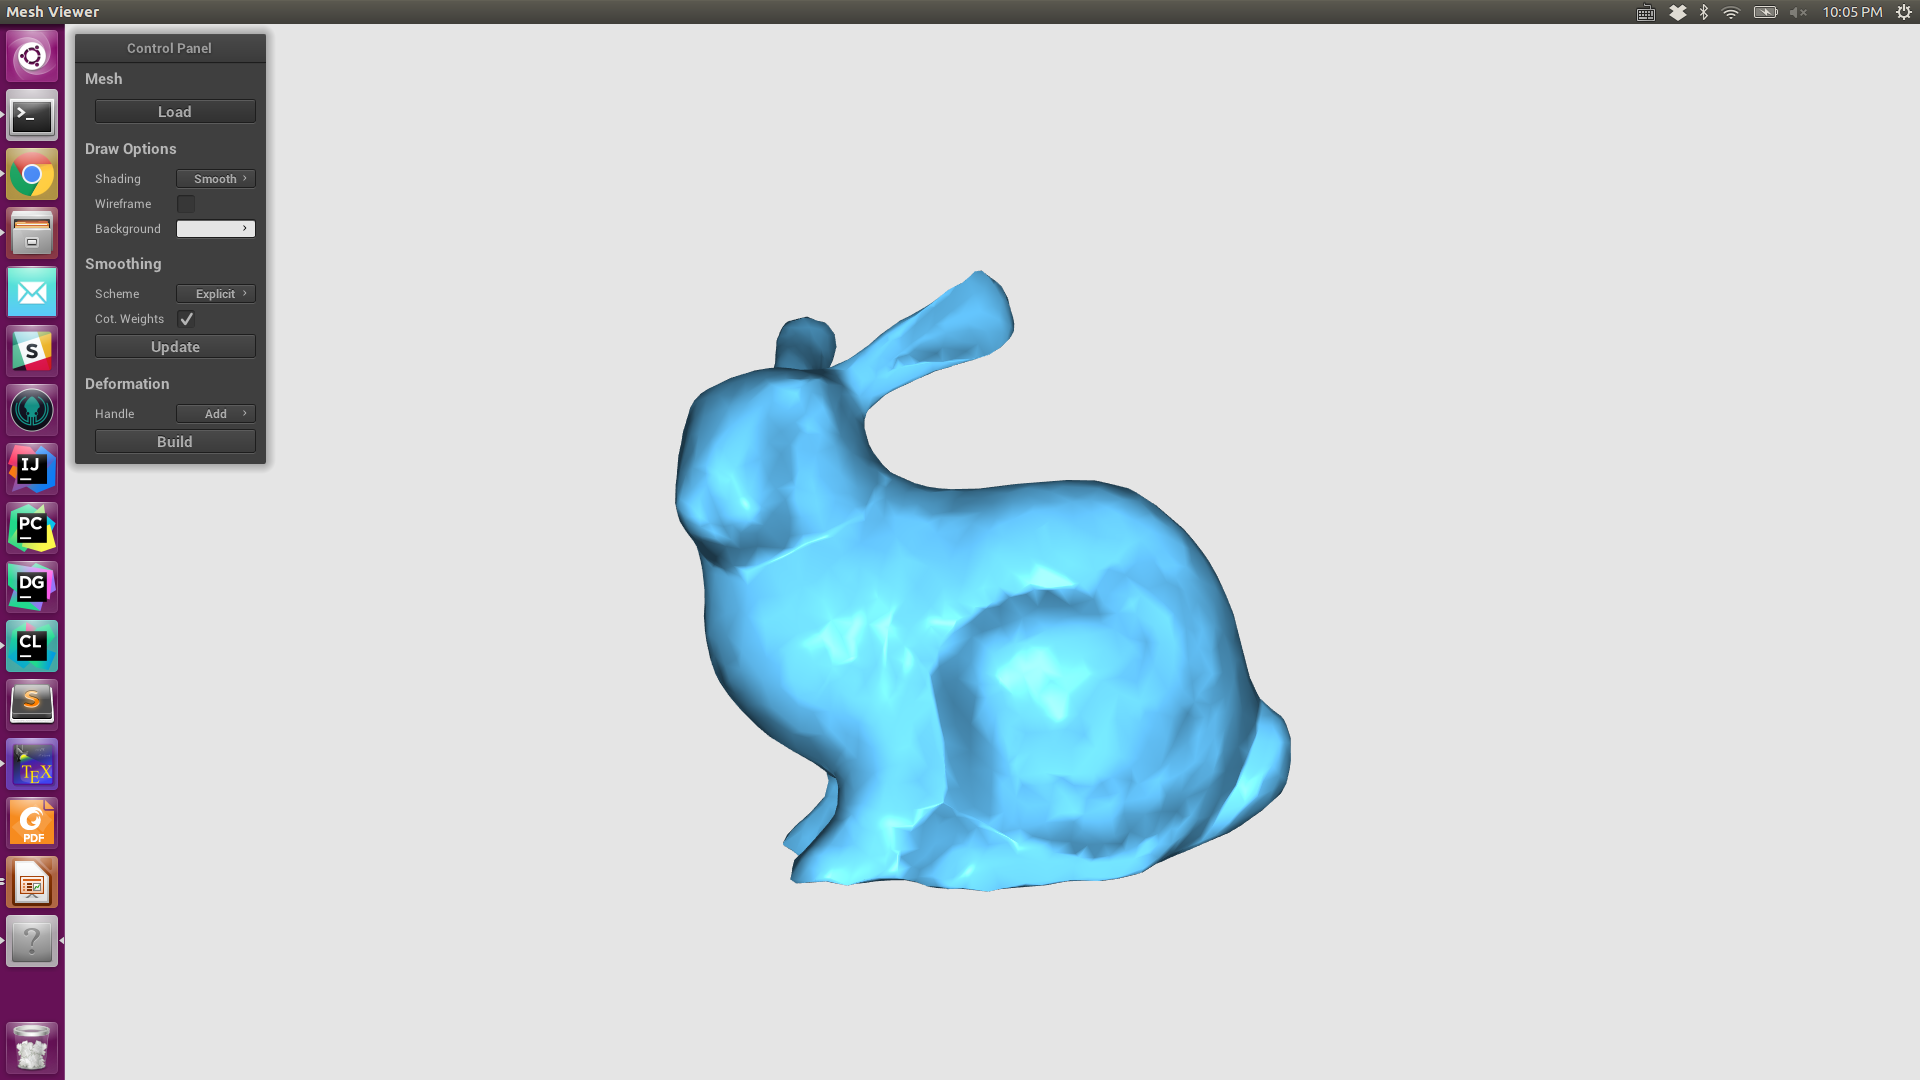
\includegraphics[width=1.0\linewidth]{bunny_ec_15.png}
	\caption{bunny after explicit cotangent weighted laplacian smoothing 15 times with $\lambda=0.5$.}
\end{figure}
\begin{figure}[H]
	\centering
	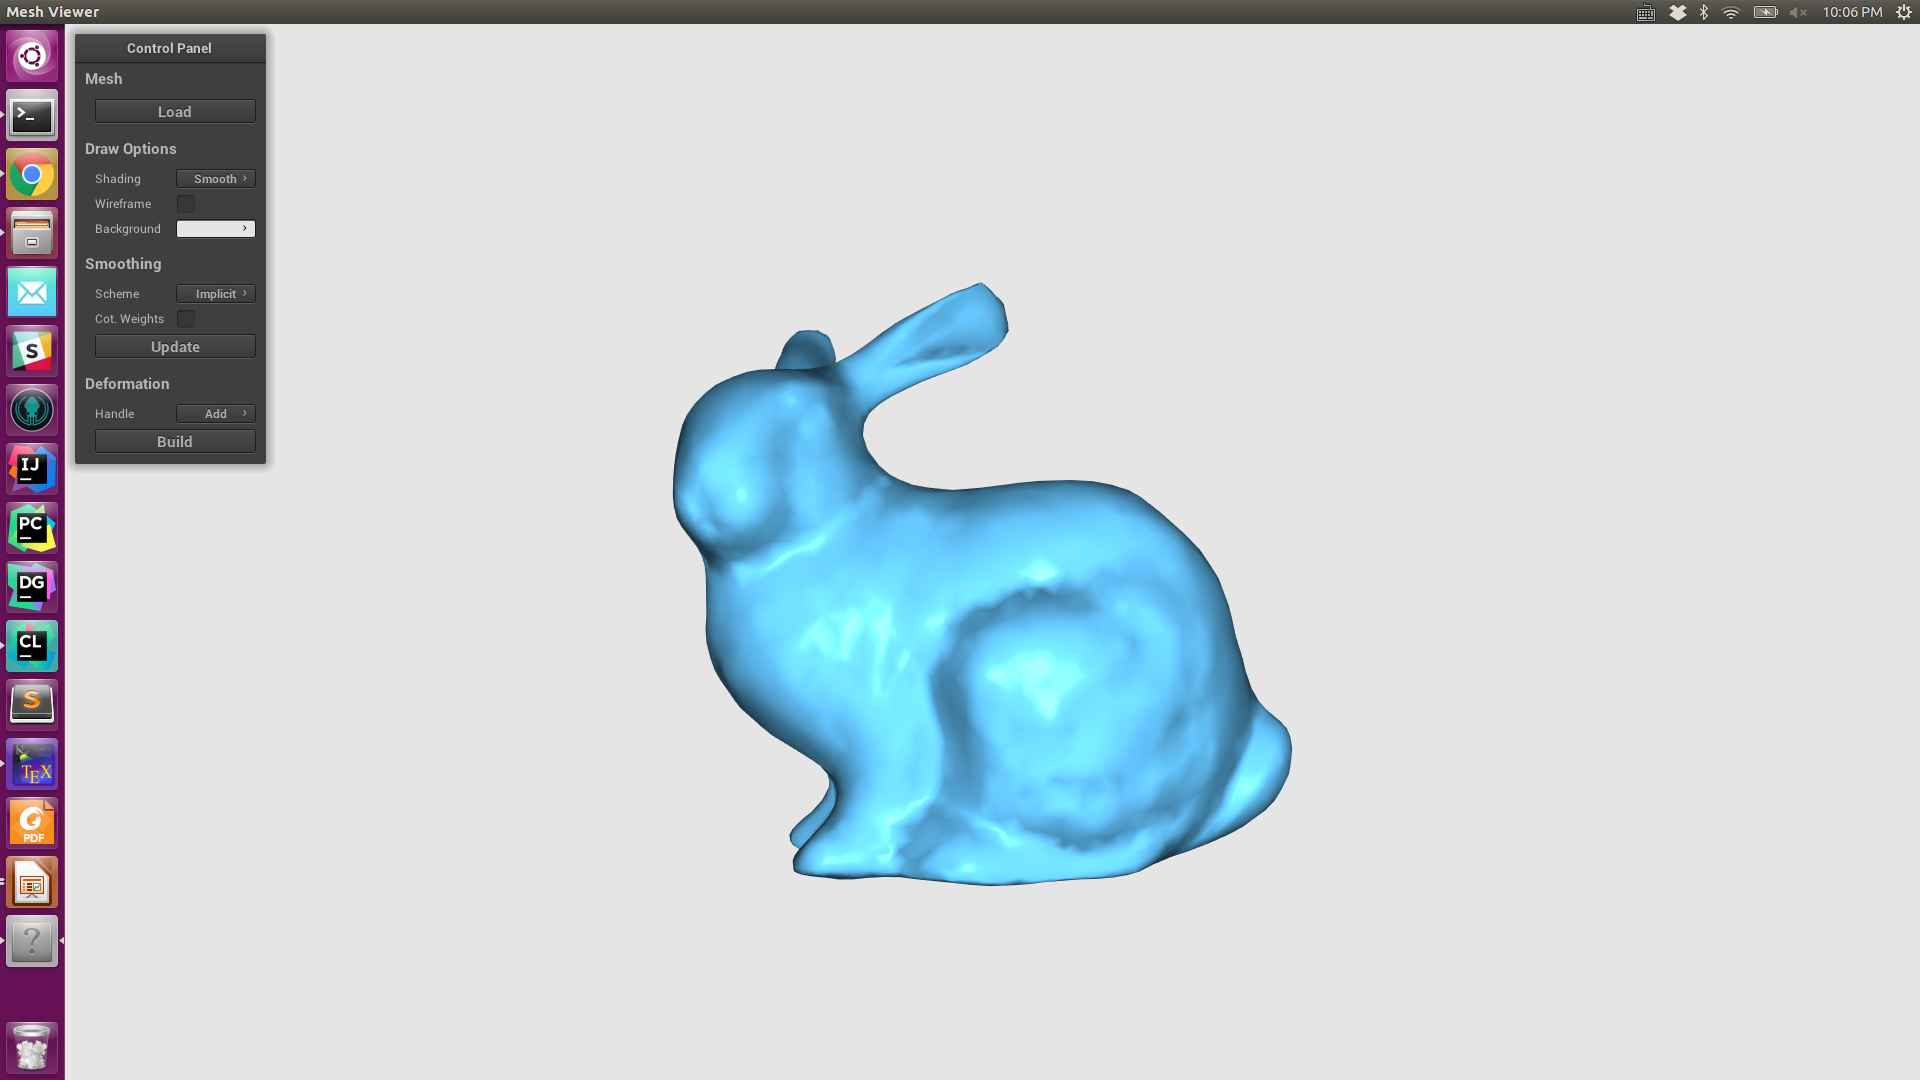
\includegraphics[width=1.0\linewidth]{bunny_in_15.png}
	\caption{bunny after implicit unweighted laplacian smoothing 15 times with $\lambda=0.5$.}
\end{figure}
\begin{figure}[H]
	\centering
	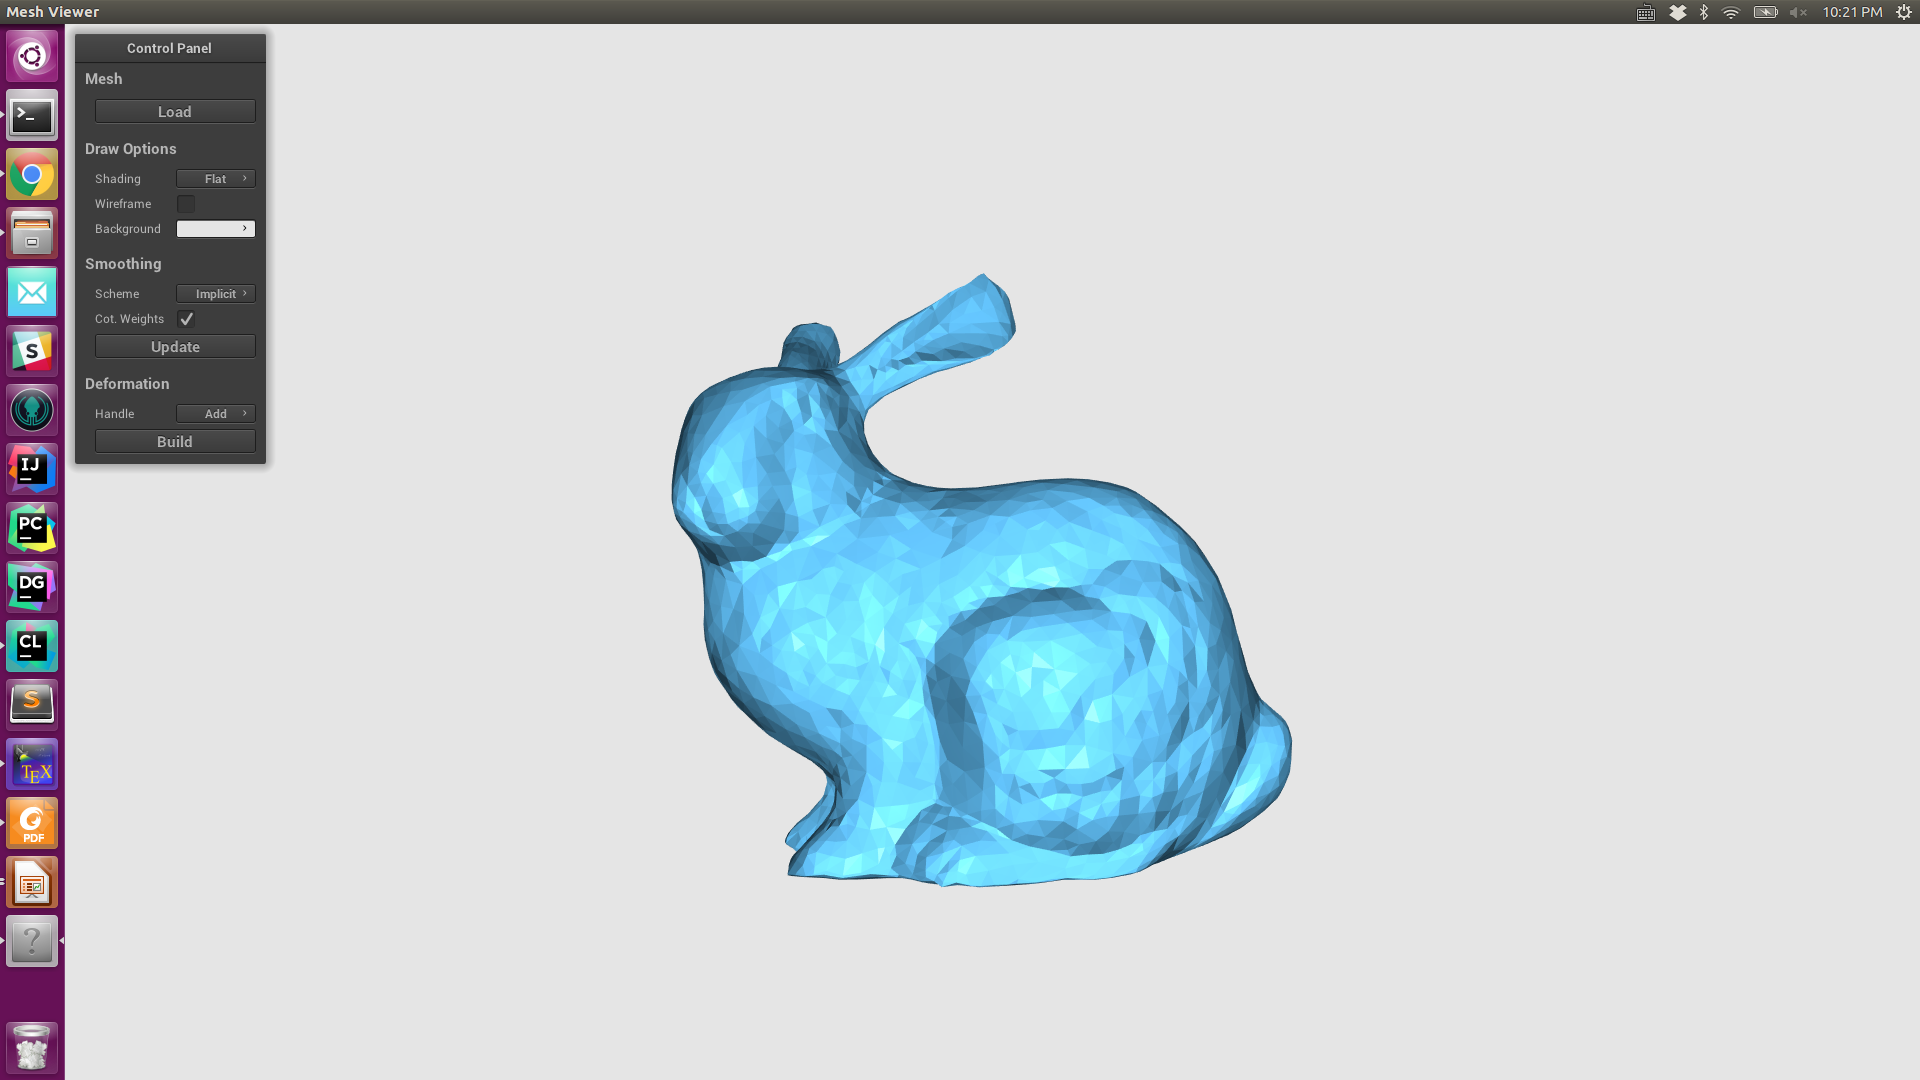
\includegraphics[width=1.0\linewidth]{bunny_ic_15.png}
	\caption{bunny after implicit cotangent weighted laplacian smoothing 15 times with $\lambda=0.5$.}
\end{figure}

\section{Laplacian Smoothing on Cube Bumpy}
\begin{figure}[H]
	\centering
	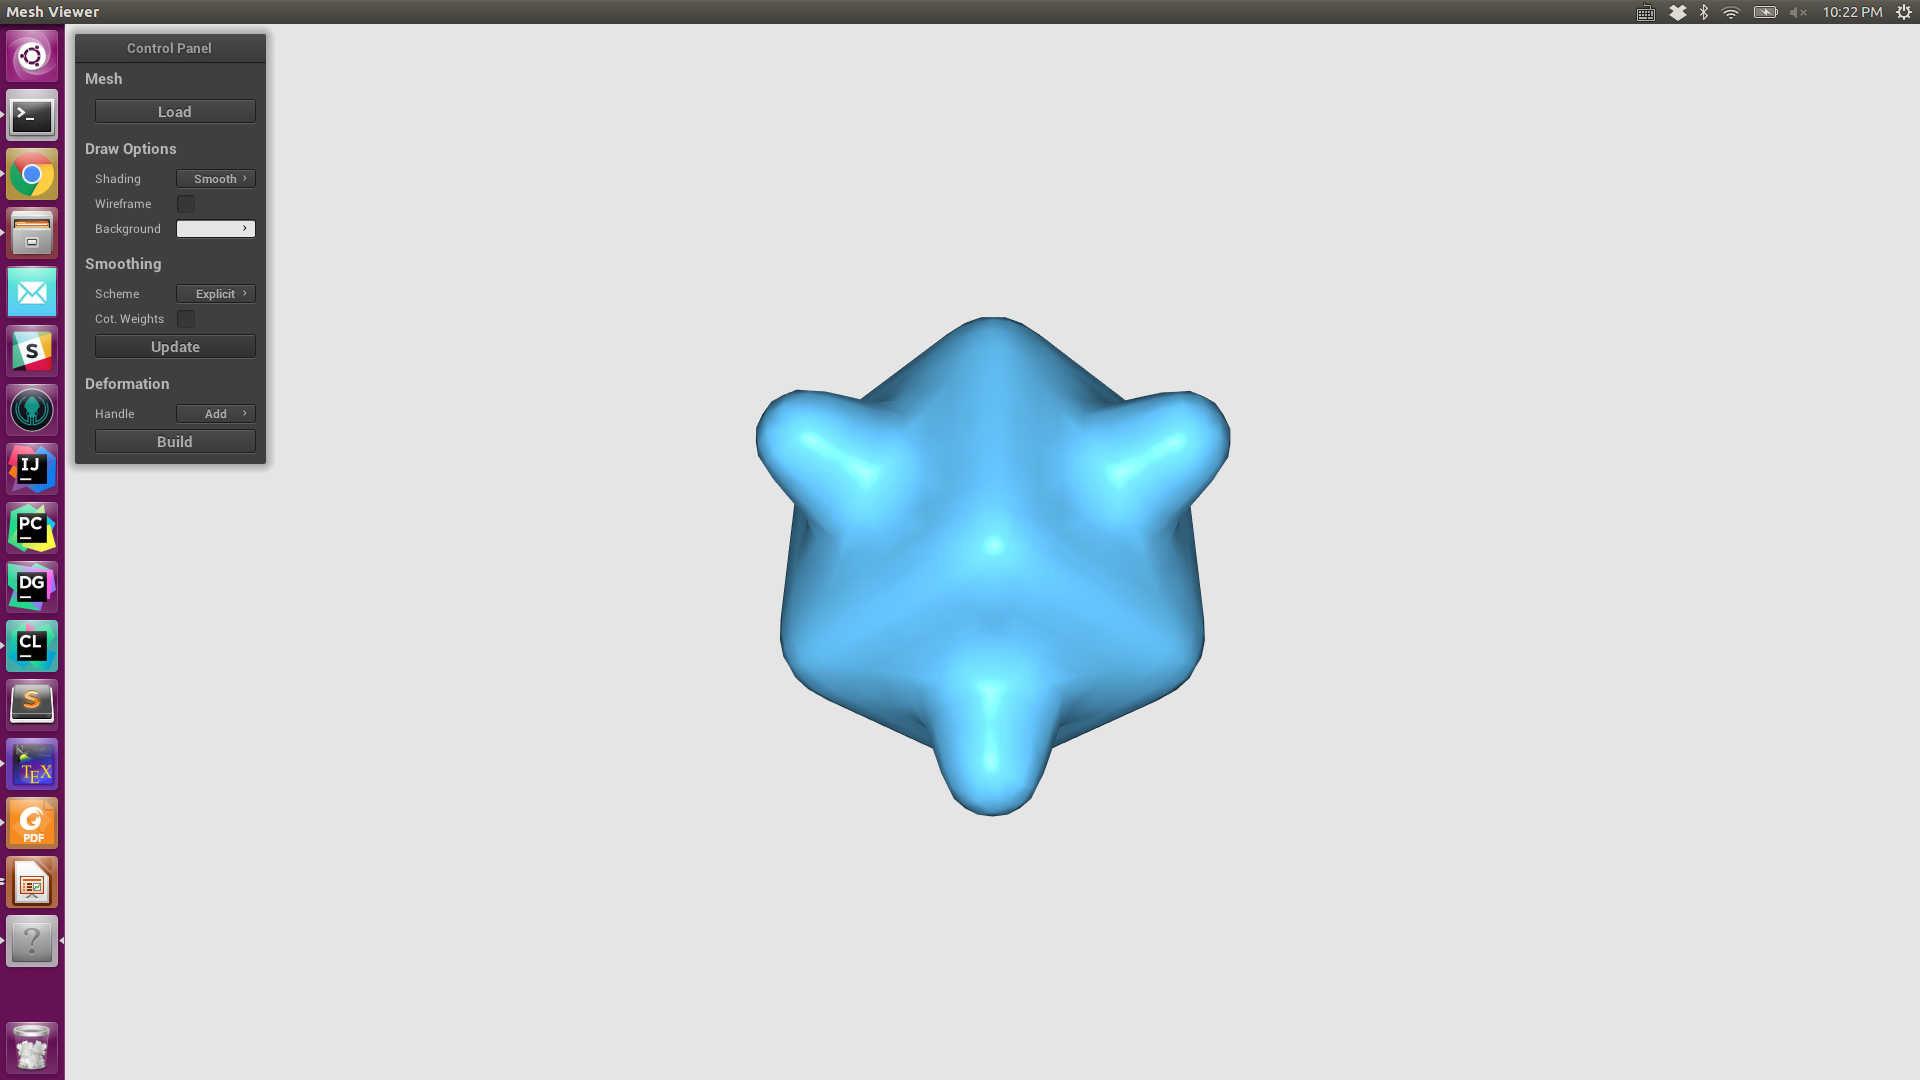
\includegraphics[width=1.0\linewidth]{cube_bumpy.png}
	\caption{original cube bumpy}
\end{figure}
\begin{figure}[H]
	\centering
	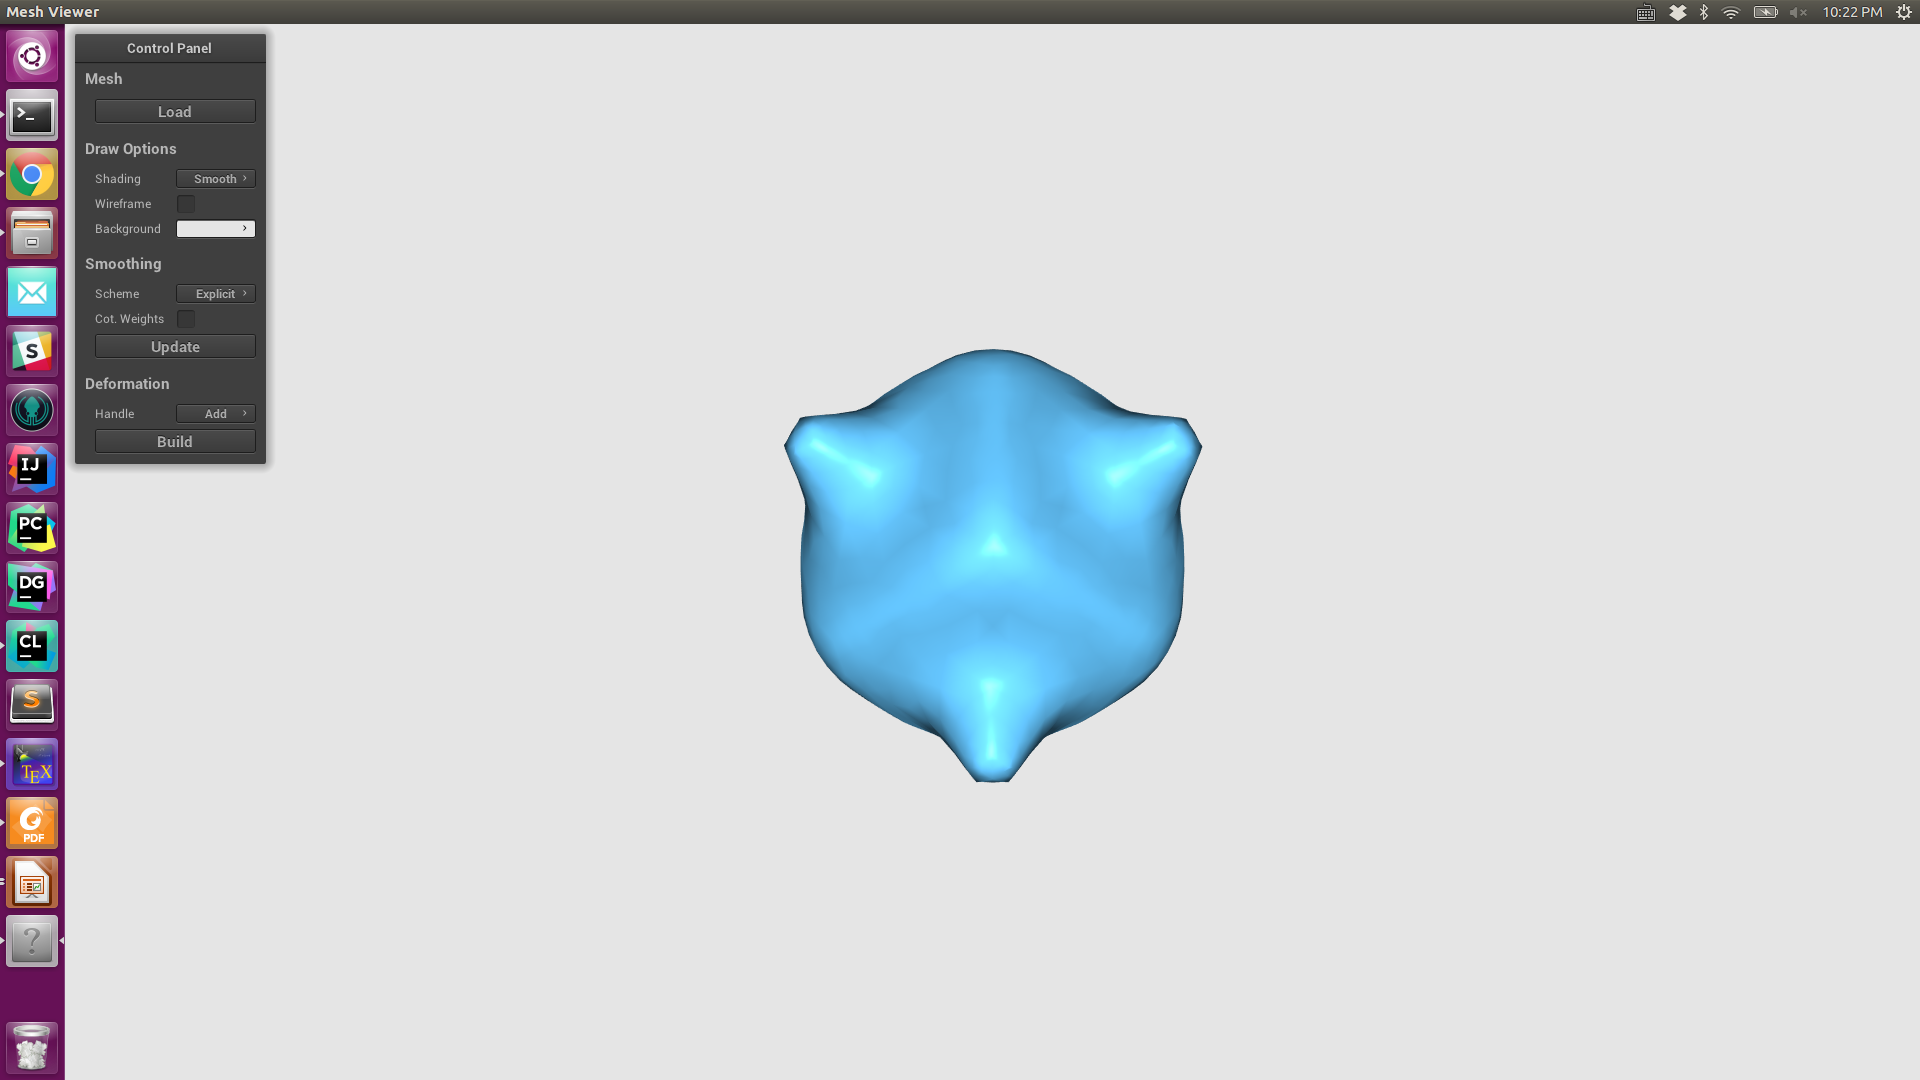
\includegraphics[width=1.0\linewidth]{cube_bumpy_en_15.png}
	\caption{cube bumpy after explicit unweighted laplacian smoothing 15 times with $\lambda=0.5$.}
\end{figure}
\begin{figure}[H]
	\centering
	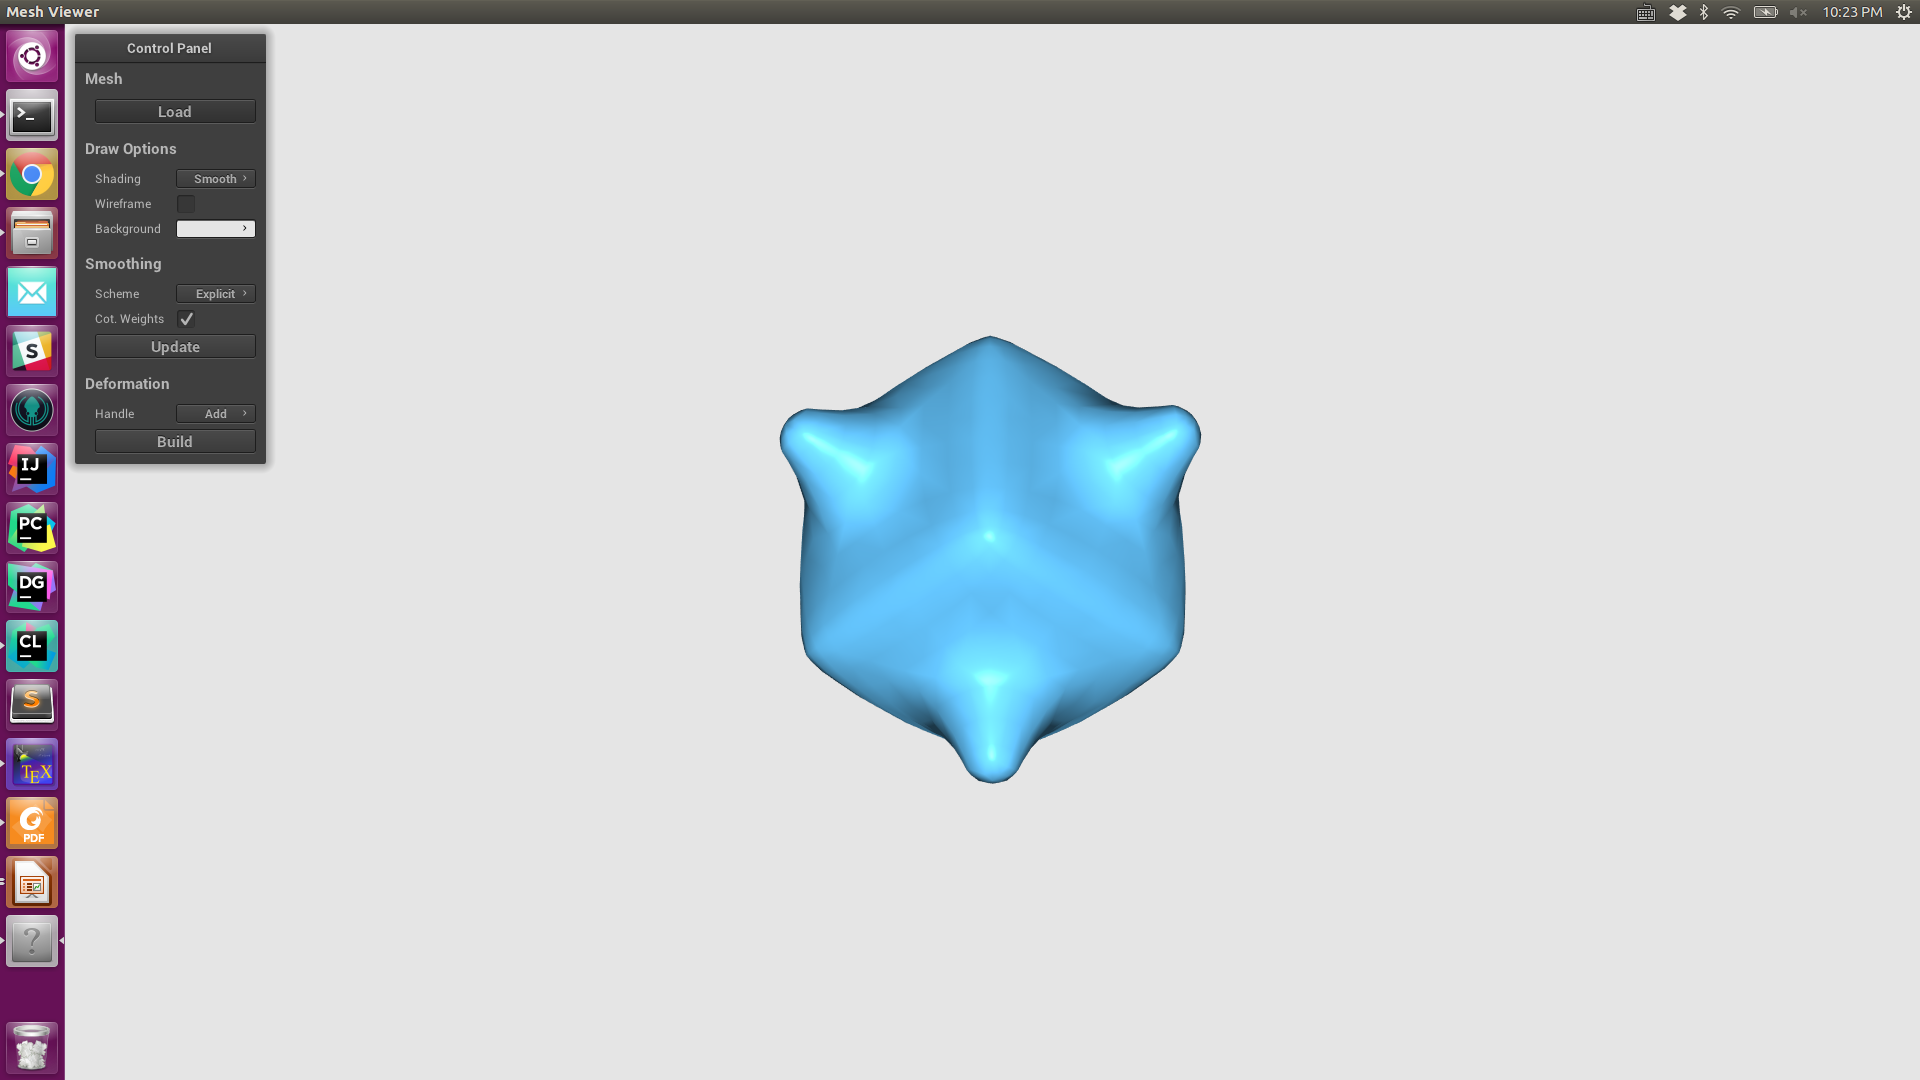
\includegraphics[width=1.0\linewidth]{cube_bumpy_ec_15.png}
	\caption{cube bumpy after explicit cotangent weighted laplacian smoothing 15 times with $\lambda=0.5$.}
\end{figure}
\begin{figure}[H]
	\centering
	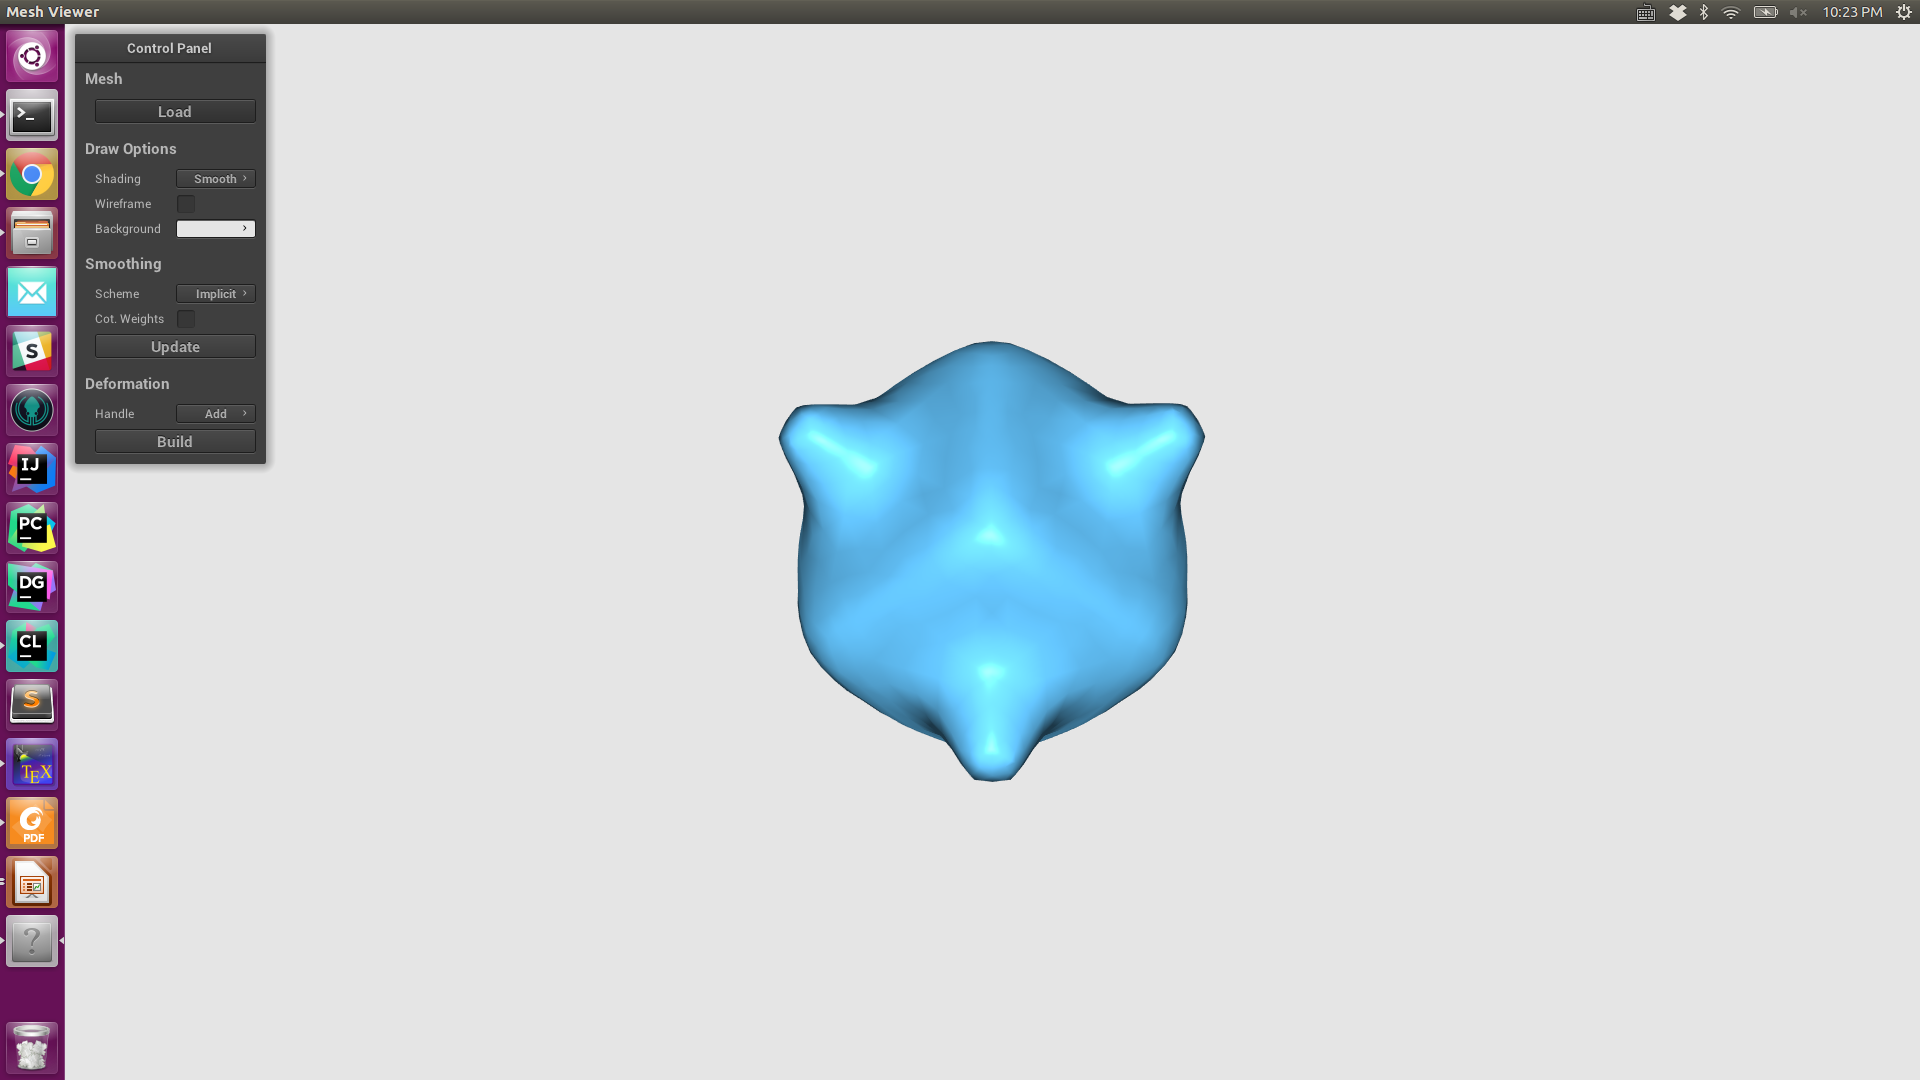
\includegraphics[width=1.0\linewidth]{cube_bumpy_in_15.png}
	\caption{cube bumpy after implicit unweighted laplacian smoothing 15 times with $\lambda=0.5$.}
\end{figure}
\begin{figure}[H]
	\centering
	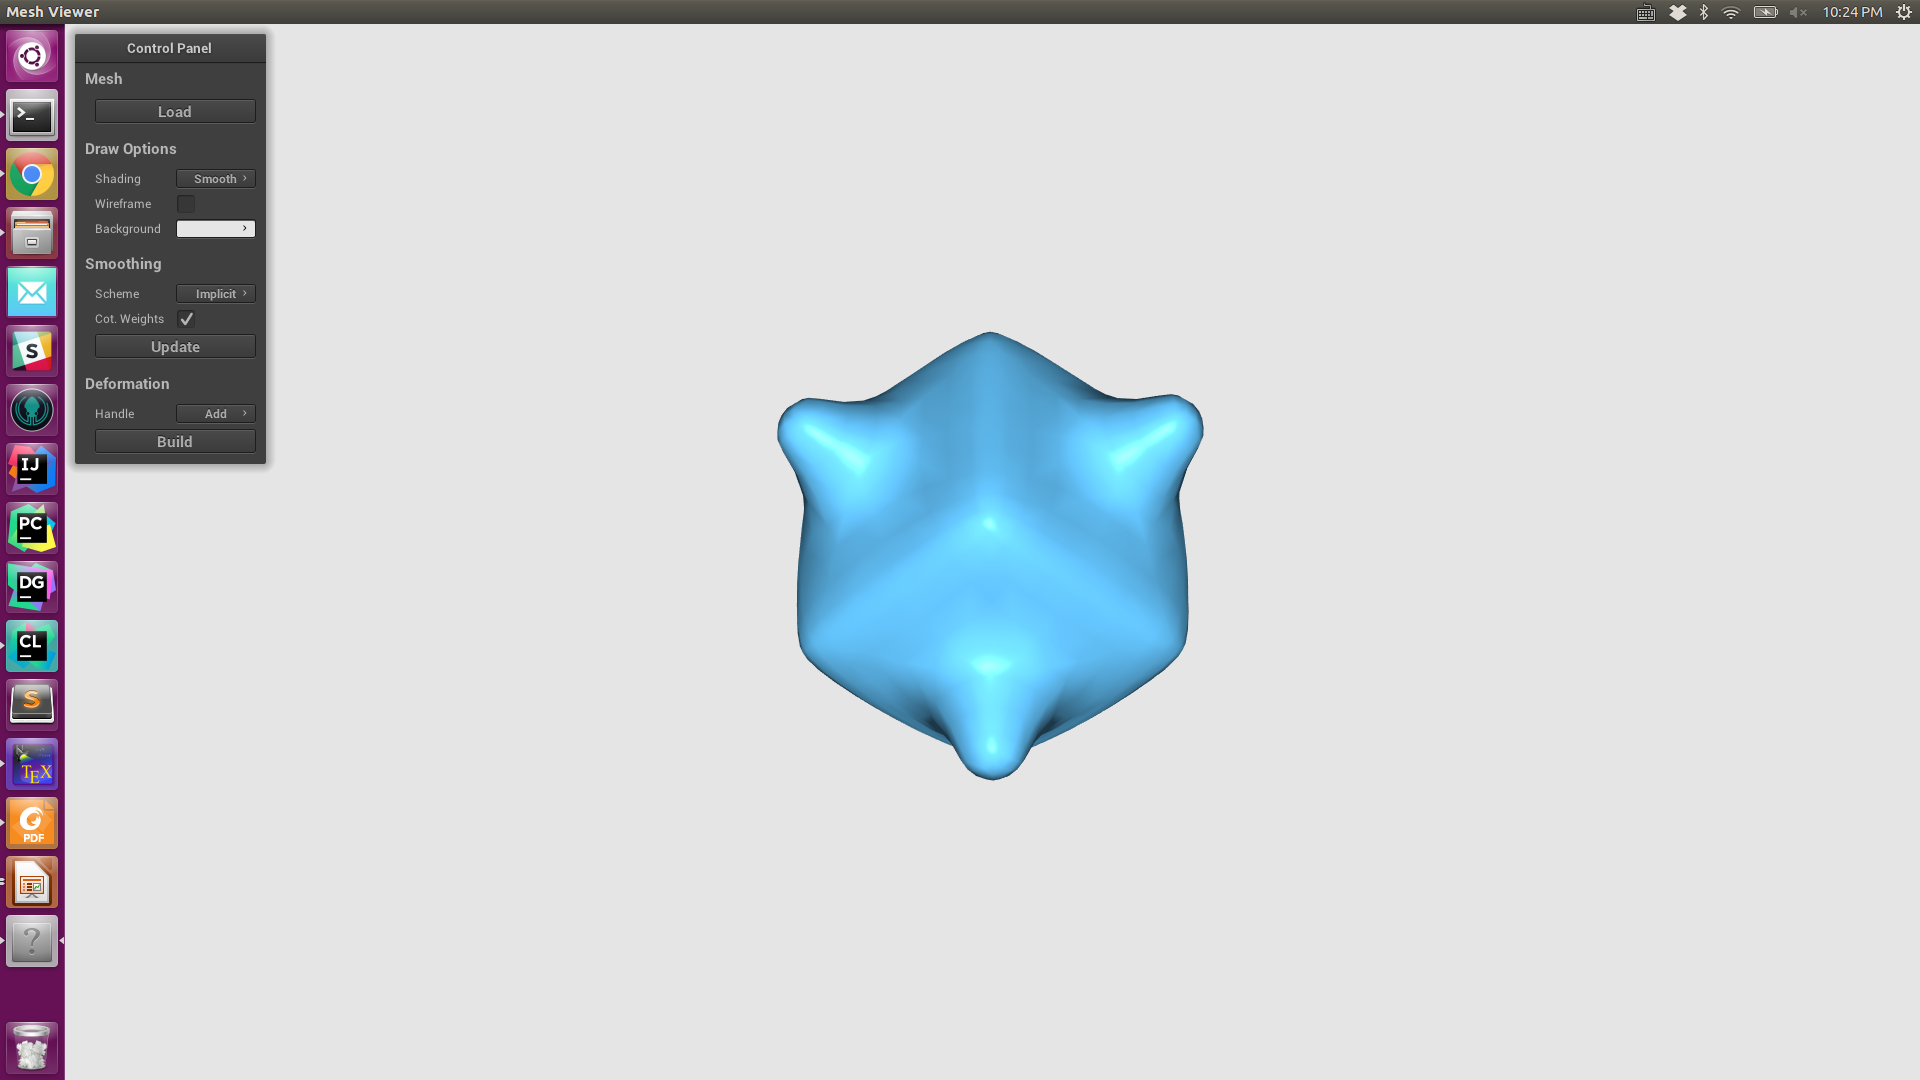
\includegraphics[width=1.0\linewidth]{cube_bumpy_ic_15.png}
	\caption{cube bumpy after implicit cotangent weighted laplacian smoothing 15 times with $\lambda=0.5$.}
\end{figure}

\section{Laplacian Smoothing on Feline}
\begin{figure}[H]
	\centering
	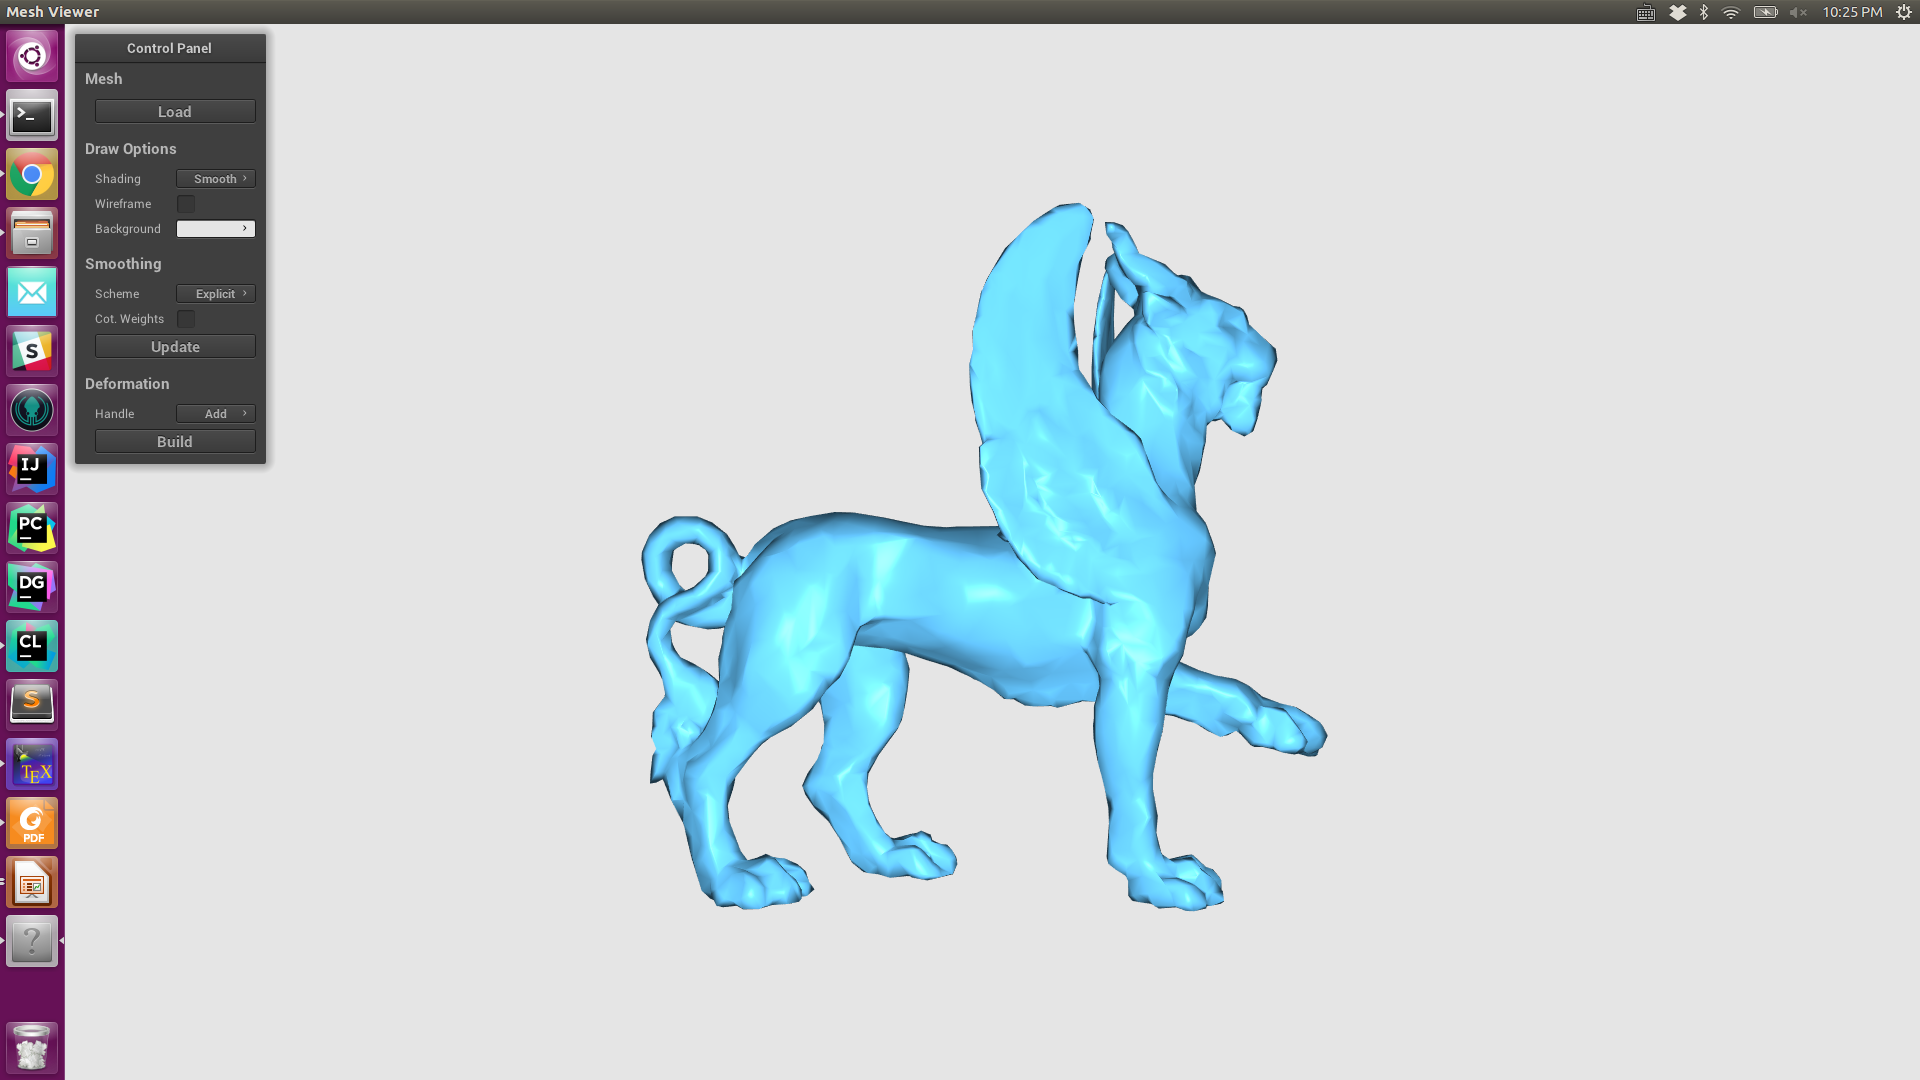
\includegraphics[width=1.0\linewidth]{feline.png}
	\caption{original feline}
\end{figure}
\begin{figure}[H]
	\centering
	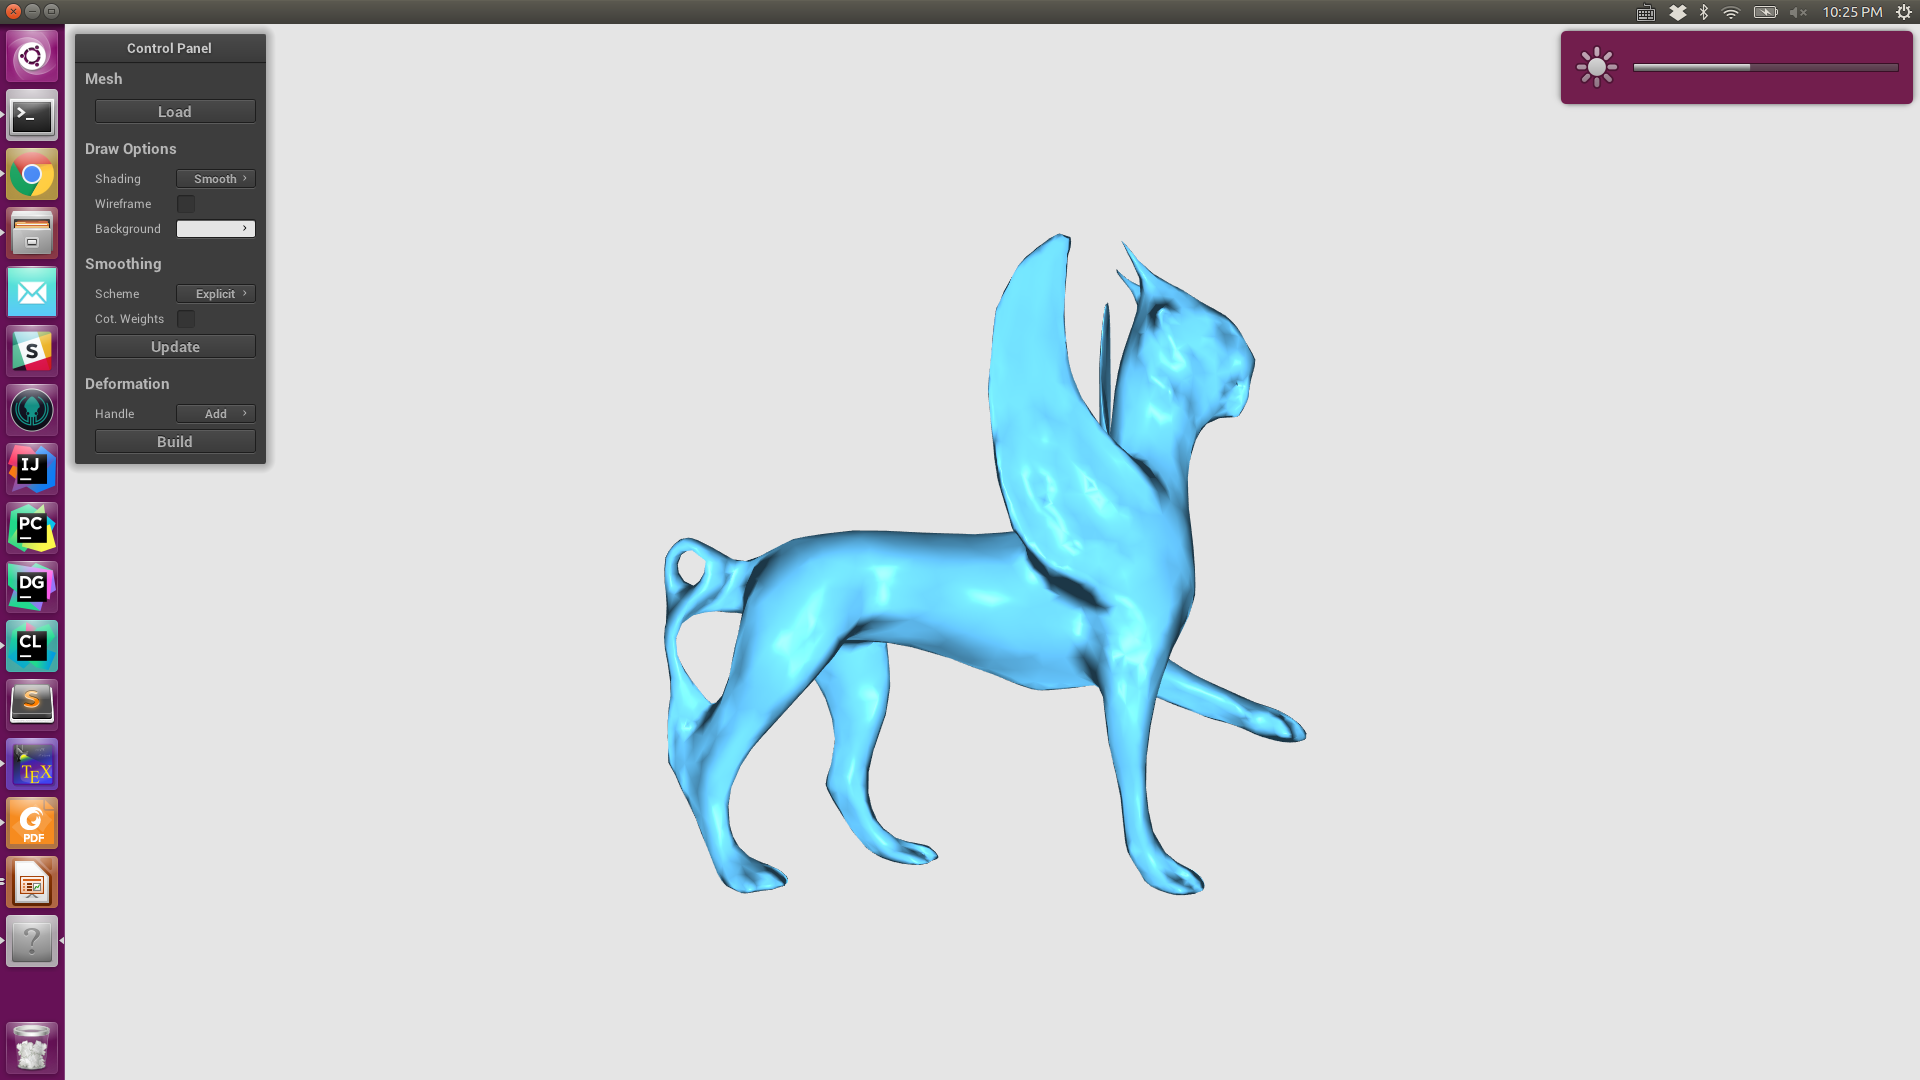
\includegraphics[width=1.0\linewidth]{feline_en_15.png}
	\caption{feline after explicit unweighted laplacian smoothing 15 times with $\lambda=0.5$.}
\end{figure}
\begin{figure}[H]
	\centering
	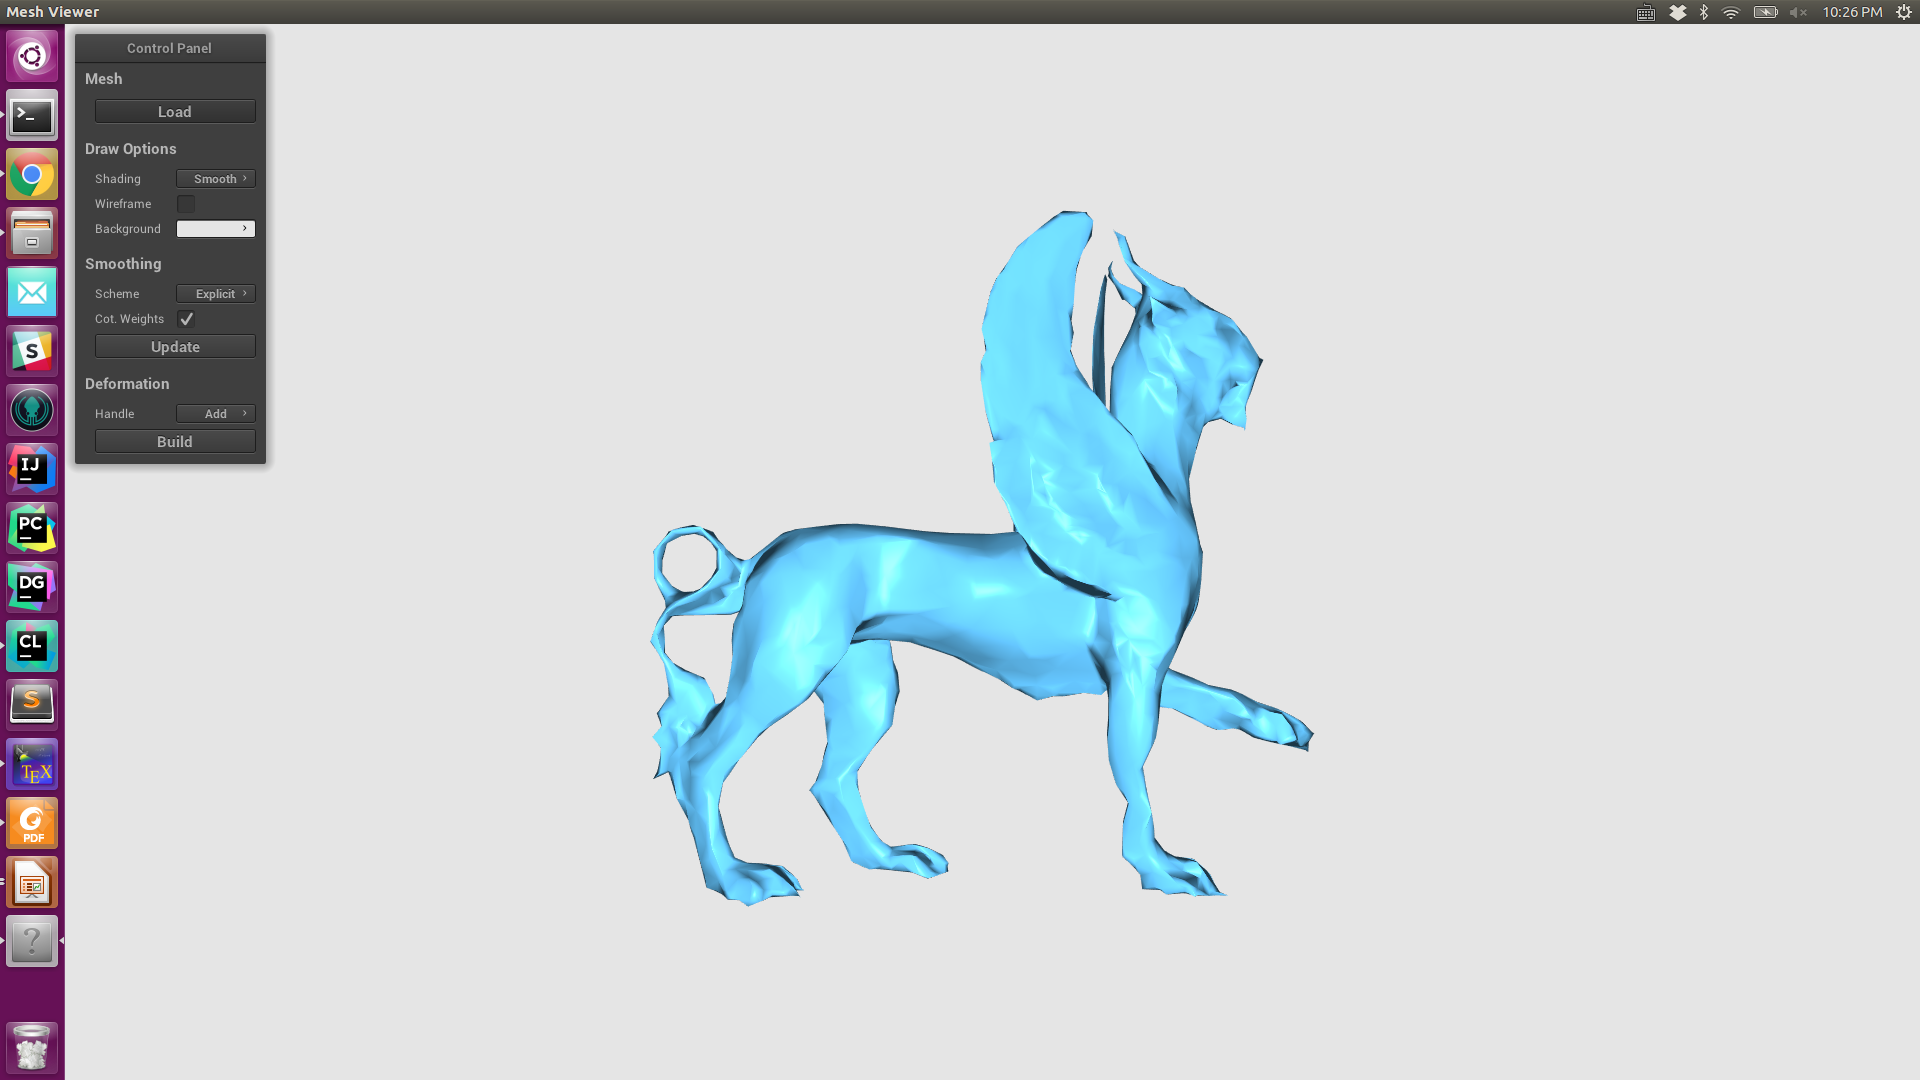
\includegraphics[width=1.0\linewidth]{feline_ec_15.png}
	\caption{feline after explicit cotangent weighted laplacian smoothing 15 times with $\lambda=0.5$.}
\end{figure}
\begin{figure}[H]
	\centering
	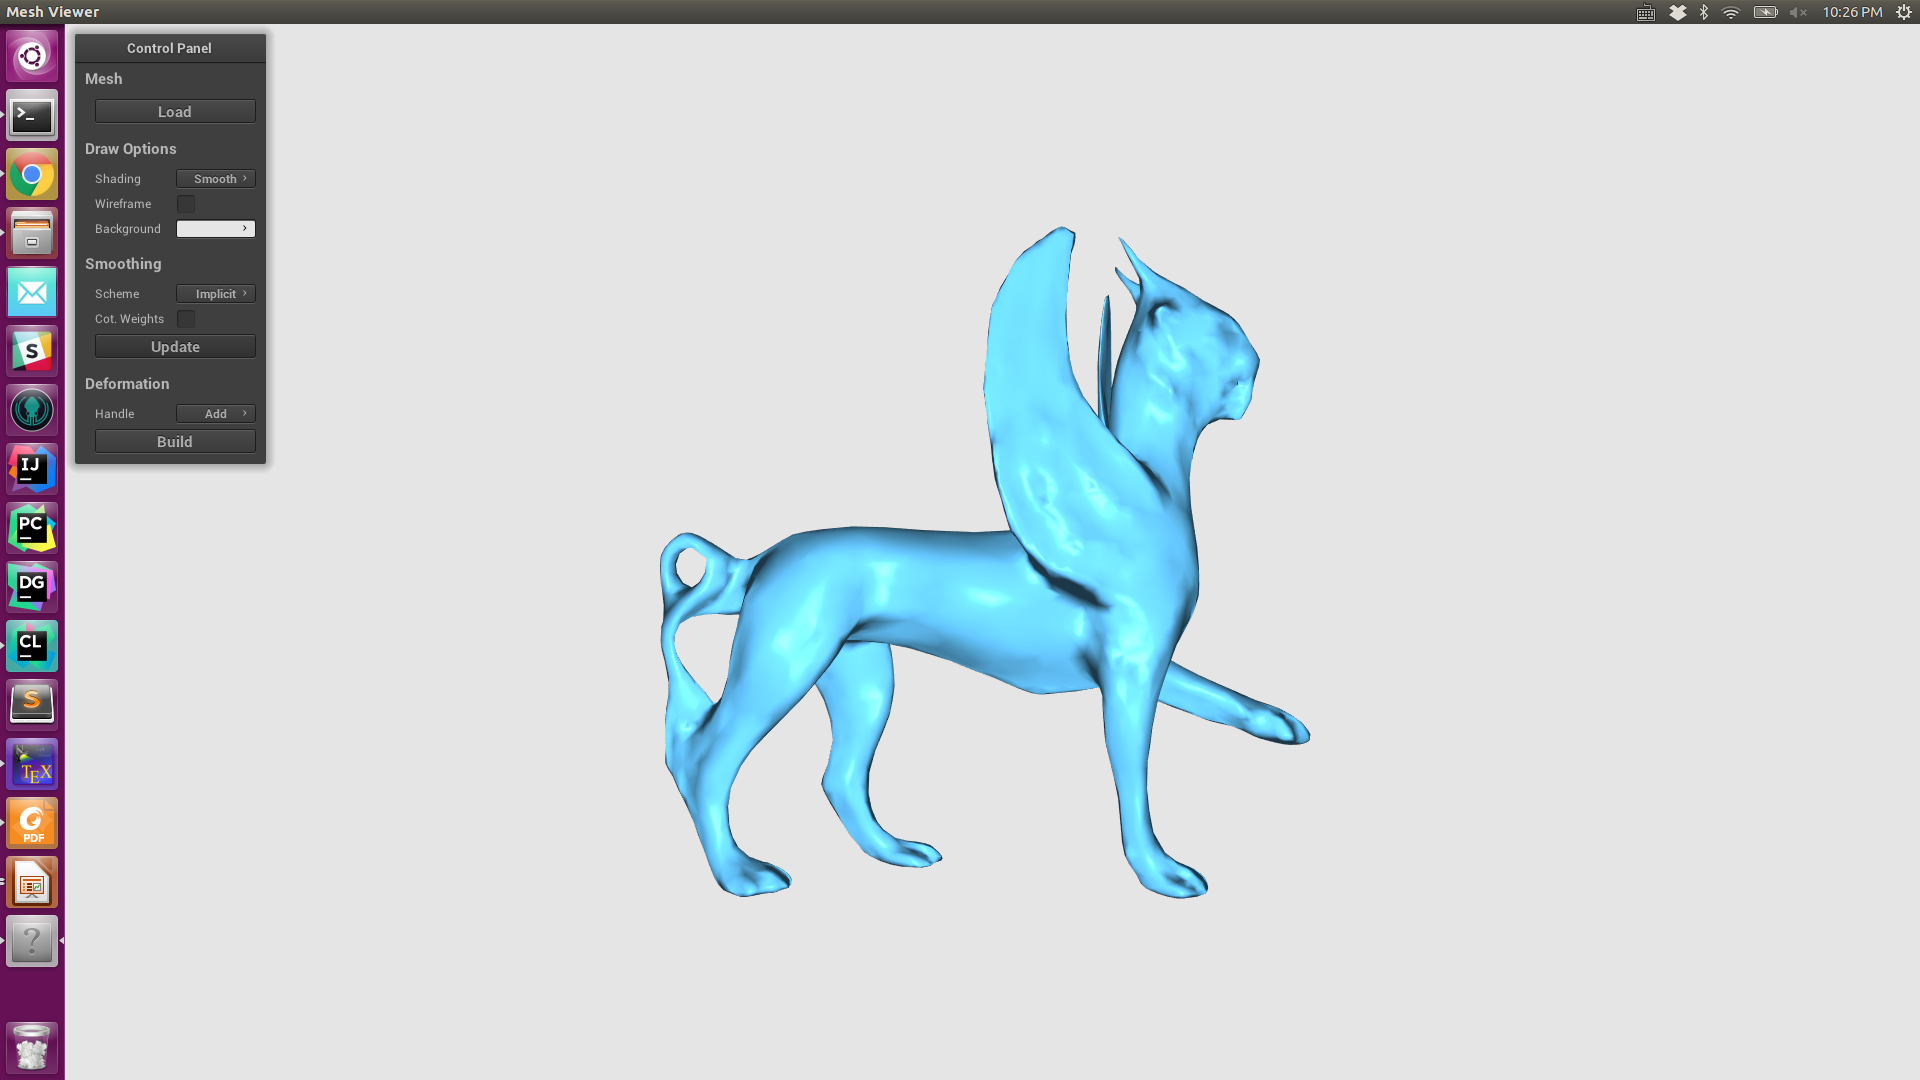
\includegraphics[width=1.0\linewidth]{feline_in_15.png}
	\caption{feline after implicit unweighted laplacian smoothing 15 times with $\lambda=0.5$.}
\end{figure}
\begin{figure}[H]
	\centering
	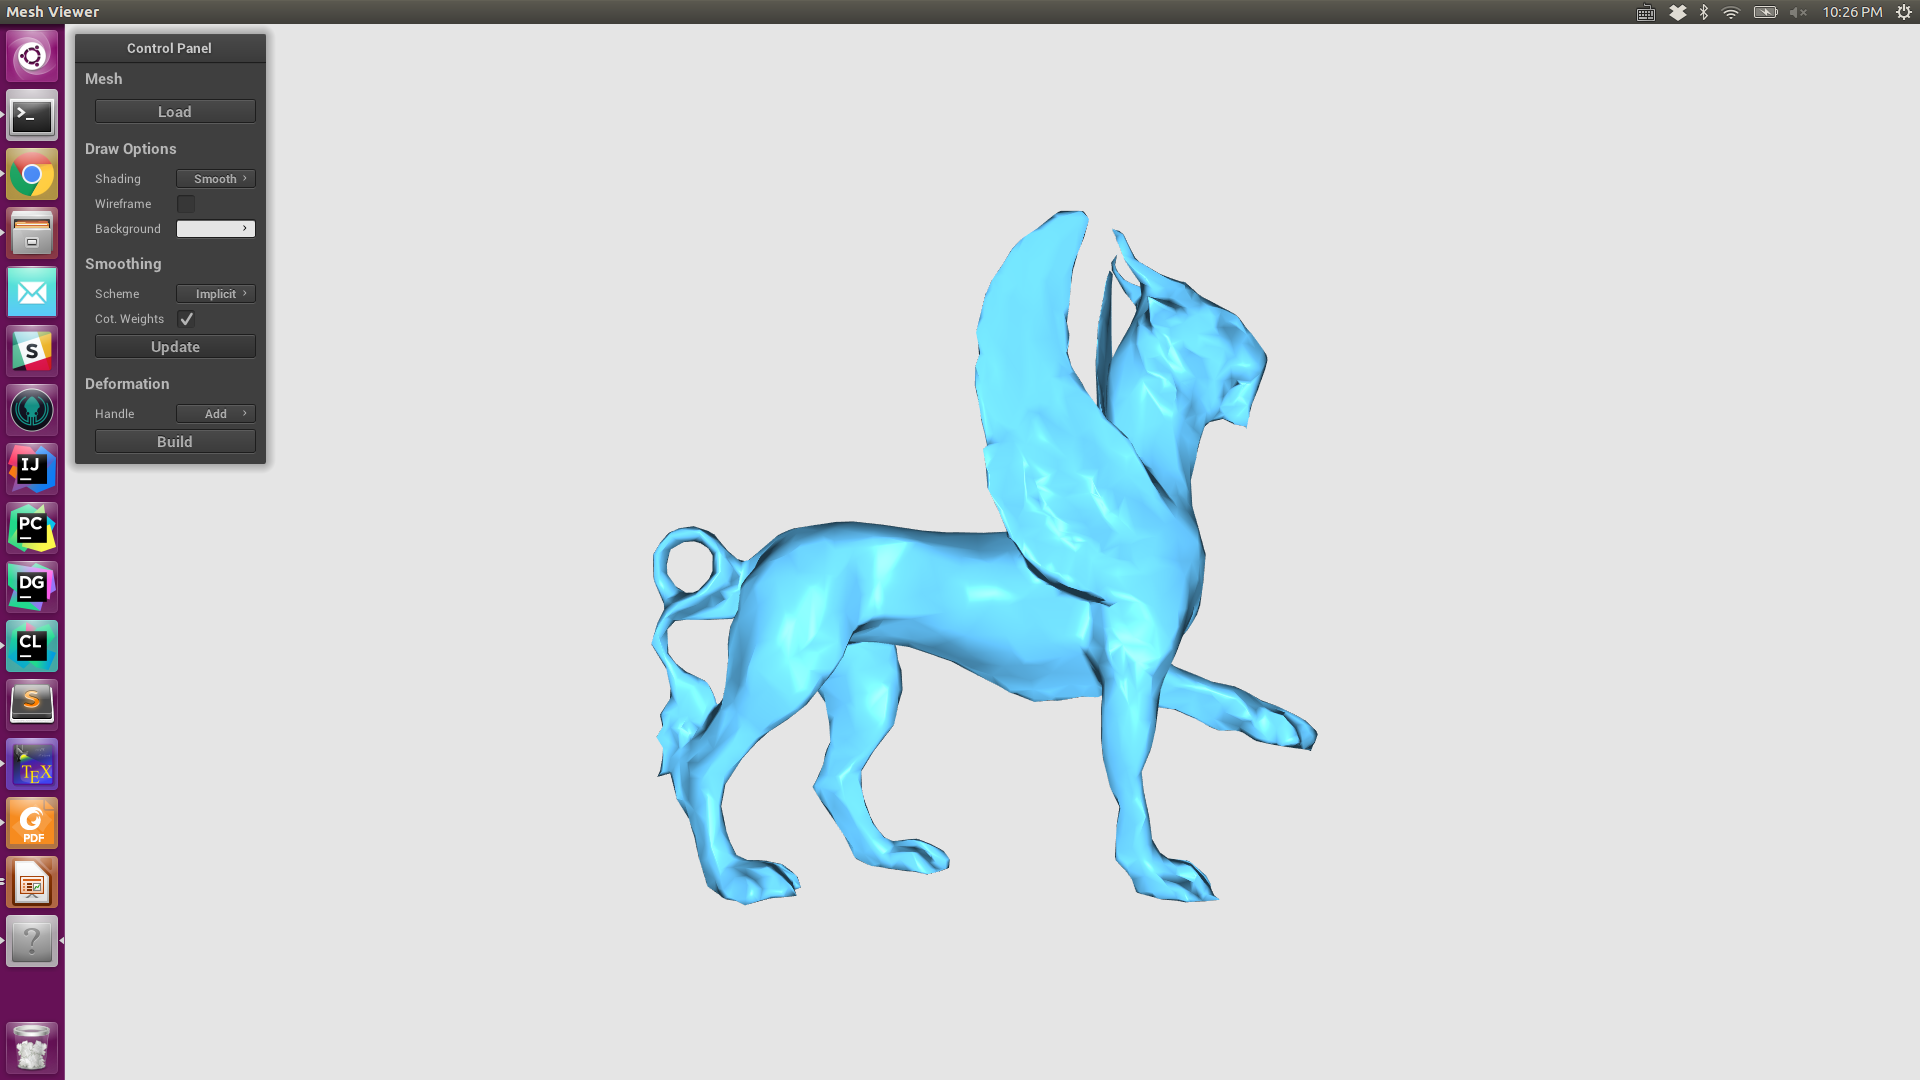
\includegraphics[width=1.0\linewidth]{feline_ic_15.png}
	\caption{feline after implicit cotangent weighted laplacian smoothing 15 times with $\lambda=0.5$.}
\end{figure}

\section{Conclusions}
Compared to the explicit scheme, the implicit scheme gives slower but gentler smoothing. To get a stable smoothing behavior, a small $\lambda<0.5$ should be used. And it is clear that the implicit scheme runs much more slower than the explicit scheme. However, since the linear equation in the implicit scheme can be solved to satisfactory precision with in around $5\sim20$ iterations, the implicit solver is still affordable fast. 

\end{document}
